% !TeX root = ../main.tex

\chapter{文獻探討}
身分系統的發展經歷了從中心化到去中心化的演變,現代身分系統設計面臨著使用者體驗、認知負擔、隱私保護和平等信任等多方面的挑戰,需要同時滿足技術創新、法規遵循和行業最佳實踐,以創造出既能滿足多樣化需求又具備足夠靈活性的解決方案,本章將探討相關文獻以深入理解這些挑戰及可能的解決途徑。
\section{身分系統的想像}
網際網路(Internet)發源於20世紀70年代,逐漸發展成為現代網際網路的基礎架構。最初,Internet的設計源自美國國防部的ARPANET計畫,旨在滿足軍事需求下的網路可用性和穩定性。因此,其初期設計基於以下假設\cite{Pekka2010HIP}:
\begin{itemize}
  \item 最終使用者至少在最低程度上相互信任。
  \item 網路由於潛在的物理攻擊而本質上不可靠。
\end{itemize}
這些假設在當時的網路環境中是合理的。但是,隨著網路的普及和應用範圍的擴大,這些假設已不再適用\cite{tomorrowinternet}。隨著Internet從一個研究驅動的項目演變為主流社會的重要組成部分,新的需求不斷湧現,不僅挑戰了原有的設計原則,還促使人們重新審視一些既有的假設。

在現代網路環境中,使用者之間的信任關係變得日益複雜。人們需要可靠的方式來識別自己和他人,以便在網路上進行交流和交易。因此,各種身分系統應運而生,以滿足網路環境中的身分識別需求。但正如Cameron\cite{cameron2005laws}所指出的,統一而理想的身分管理系統實際上並不存在。身分系統涉及的範疇廣泛而複雜,個人與組織之間存在多樣化且往往相互衝突的需求,試圖通過單一標準來限制或規範這些需求是不切實際的。

例如,終端使用者可能希望自由地訪問和分享信息,而內容提供商和知識產權持有者則希望保護其知識產權。政府可能希望監管某些網絡活動以維護社會秩序,而使用者和隱私倡導者則強調個人隱私的重要性。這種複雜的利益衝突導致了諸如網絡中立性、數據隱私、內容審查等一系列熱點問題的出現\cite{Wu2003NetworkNeutrality}。

面對這種複雜的網絡環境,Blumenthal\cite{Blumenthal2001RethinkingThe}認為確保設計上的一般性、彈性與開放性至關重要。他設想的未來充滿衝突:企業的管理者和被管理者爭論分紅,垃圾郵件的發送者和接收者爭論各自的困難。在這個網路世界中,不同身分的參與者沒有絕對的贏家,也沒有天生的失敗者。理想的系統應該通過所有使用者不斷的爭論和互動逐漸形成。

這種新的設計思路不僅需要考慮技術因素,還需要權衡經濟、社會、法律等多方面的因素。正如Lessig\cite{lessig2000}所言,"程式碼就是法則"("Code is Law")。軟體設計本身就在表達某種價值觀,人們需要縝密的思考,結合對未來世界的想像,才能創造出足以改變網路環境既有困境的身分系統。

總而言之,現代網路環境的變遷對身分系統提出了新的挑戰,這些挑戰不僅來自技術層面,還涉及社會、文化和法律等多個方面。為了應對這些挑戰,人們需要重新思考身分系統的設計理念,尋找一種既能適應當前多樣化需求,又能為未來發展預留足夠靈活性的解決方案。
\section{身分系統的迭代}
% todo 加表格比較每個階段的優缺點
身分系統的設計經歷了多個階段的演變,每個階段都試圖解決特定的問題,同時也帶來了新的挑戰。本節將介紹不同世代的身分系統設計,以說明彼此衝突的需求和技術限制,並為後續討論提供背景。
\subsection{中心化身分}
\begin{figure}
  \centering
  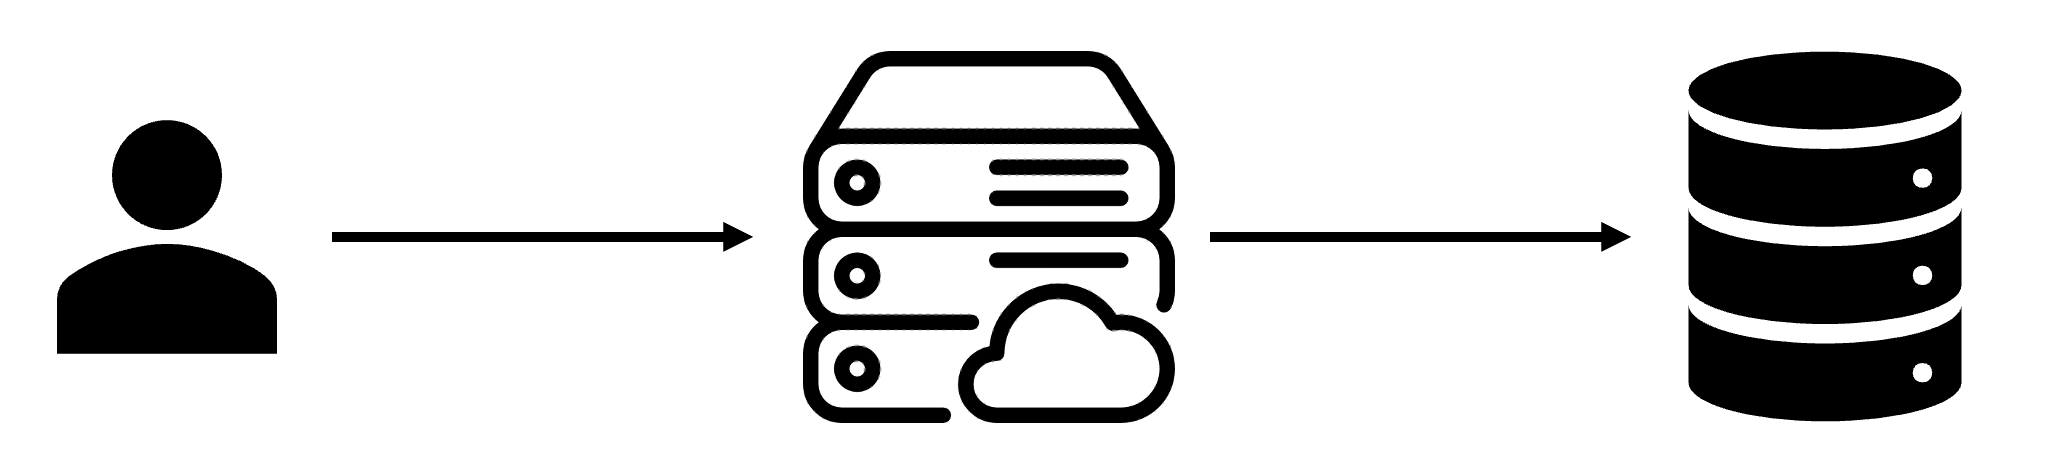
\includegraphics[width=\linewidth,keepaspectratio]{figures/mid-identity.png}
  \caption{中心化身分}
  \label{fig:mid-identity}
\end{figure}
中心化身分系統如圖\ref{fig:mid-identity}是最早期的身分管理方案,由同一位管理者操作和存儲所有使用者資訊,在企業和政府機構中廣泛應用。典型例子包括活動目錄(Windows Active Directory, AD)和輕量級目錄訪問協議(Lightweight Directory Access Protocol, LDAP)\cite{microsoft2021active, sermersheim2006lightweight}。這類系統的主要優勢在於其集中管理的特性,便於系統管理員進行使用者管理和權限控制,同時確保組織內部身分信息的一致性和及時更新。然而,中心化身分系統也面臨著諸多挑戰,如單點故障風險、隱私保護問題,以及跨組織可遷移性差等。使用者通常需要為每個服務創建單獨帳戶,這不僅增加了認知負擔\cite{josang2007security},還導致使用者身分被服務提供商完全控制,缺乏自主權。
\subsection{聯合身分}
\begin{figure}
  \centering
  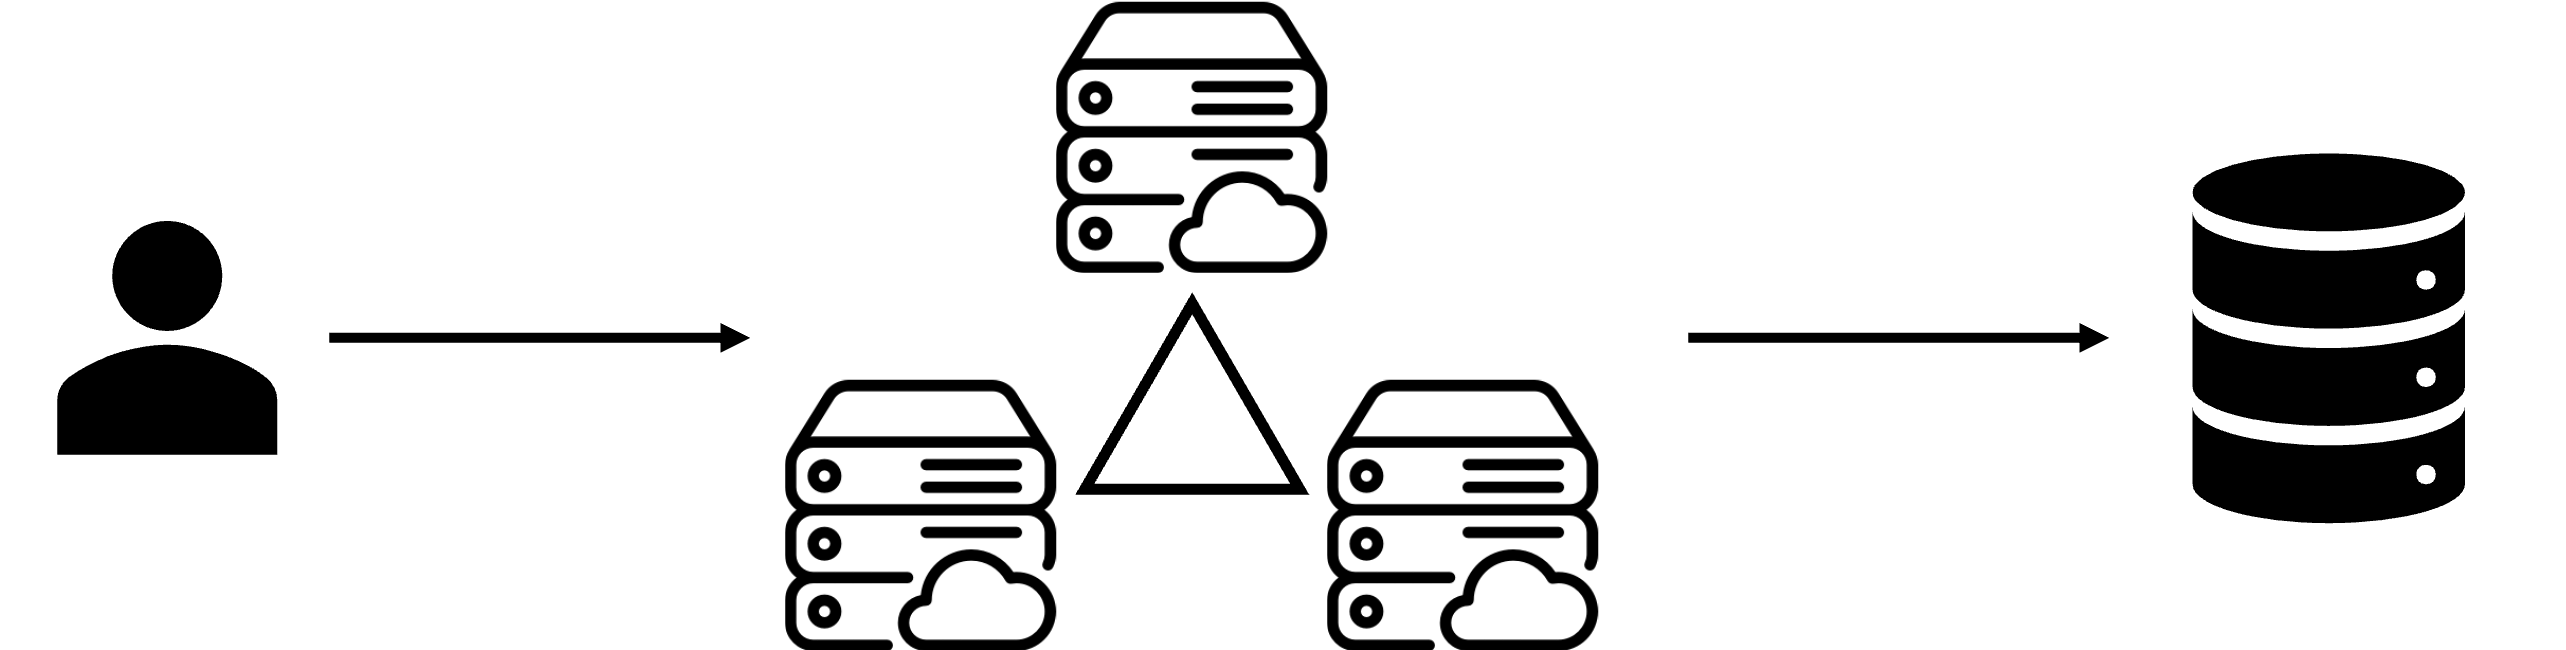
\includegraphics[width=\linewidth,keepaspectratio]{figures/group-identity.png}
  \caption{聯合身分}
  \label{fig:group-identity}
\end{figure}
主要為了解決同一個使用者擁有太多身分的認知負擔,聯合身分系統如圖\ref{fig:group-identity}允許不同組織間共享身分信息,代表性技術包括安全斷言標記語言(Security Assertion Markup Language, SAML)和 WS-Federation \cite{oasis2005security, goodner2009web}。這種模式的出現大大改善了使用者體驗,實現了單點登錄(Single sign-on,SSO),減少了密碼疲勞問題。聯合身分系統促進了組織間的協作和資源共享,同時也降低了重複身分管理的運營成本。但是,這種模式也帶來了隱私方面的挑戰\cite{ahn2007user},如使用者信息在多個服務提供商間共享可能違反《通用資料保護規則》(General Data Protection Regulation,GDPR)\cite{GDPR2016}等隱私法規。此外,實施和維護聯合身分系統的技術複雜度較高,參與組織之間需要建立並維護信任關係。
\subsection{使用者中心的身分}
\begin{figure}
  \centering
  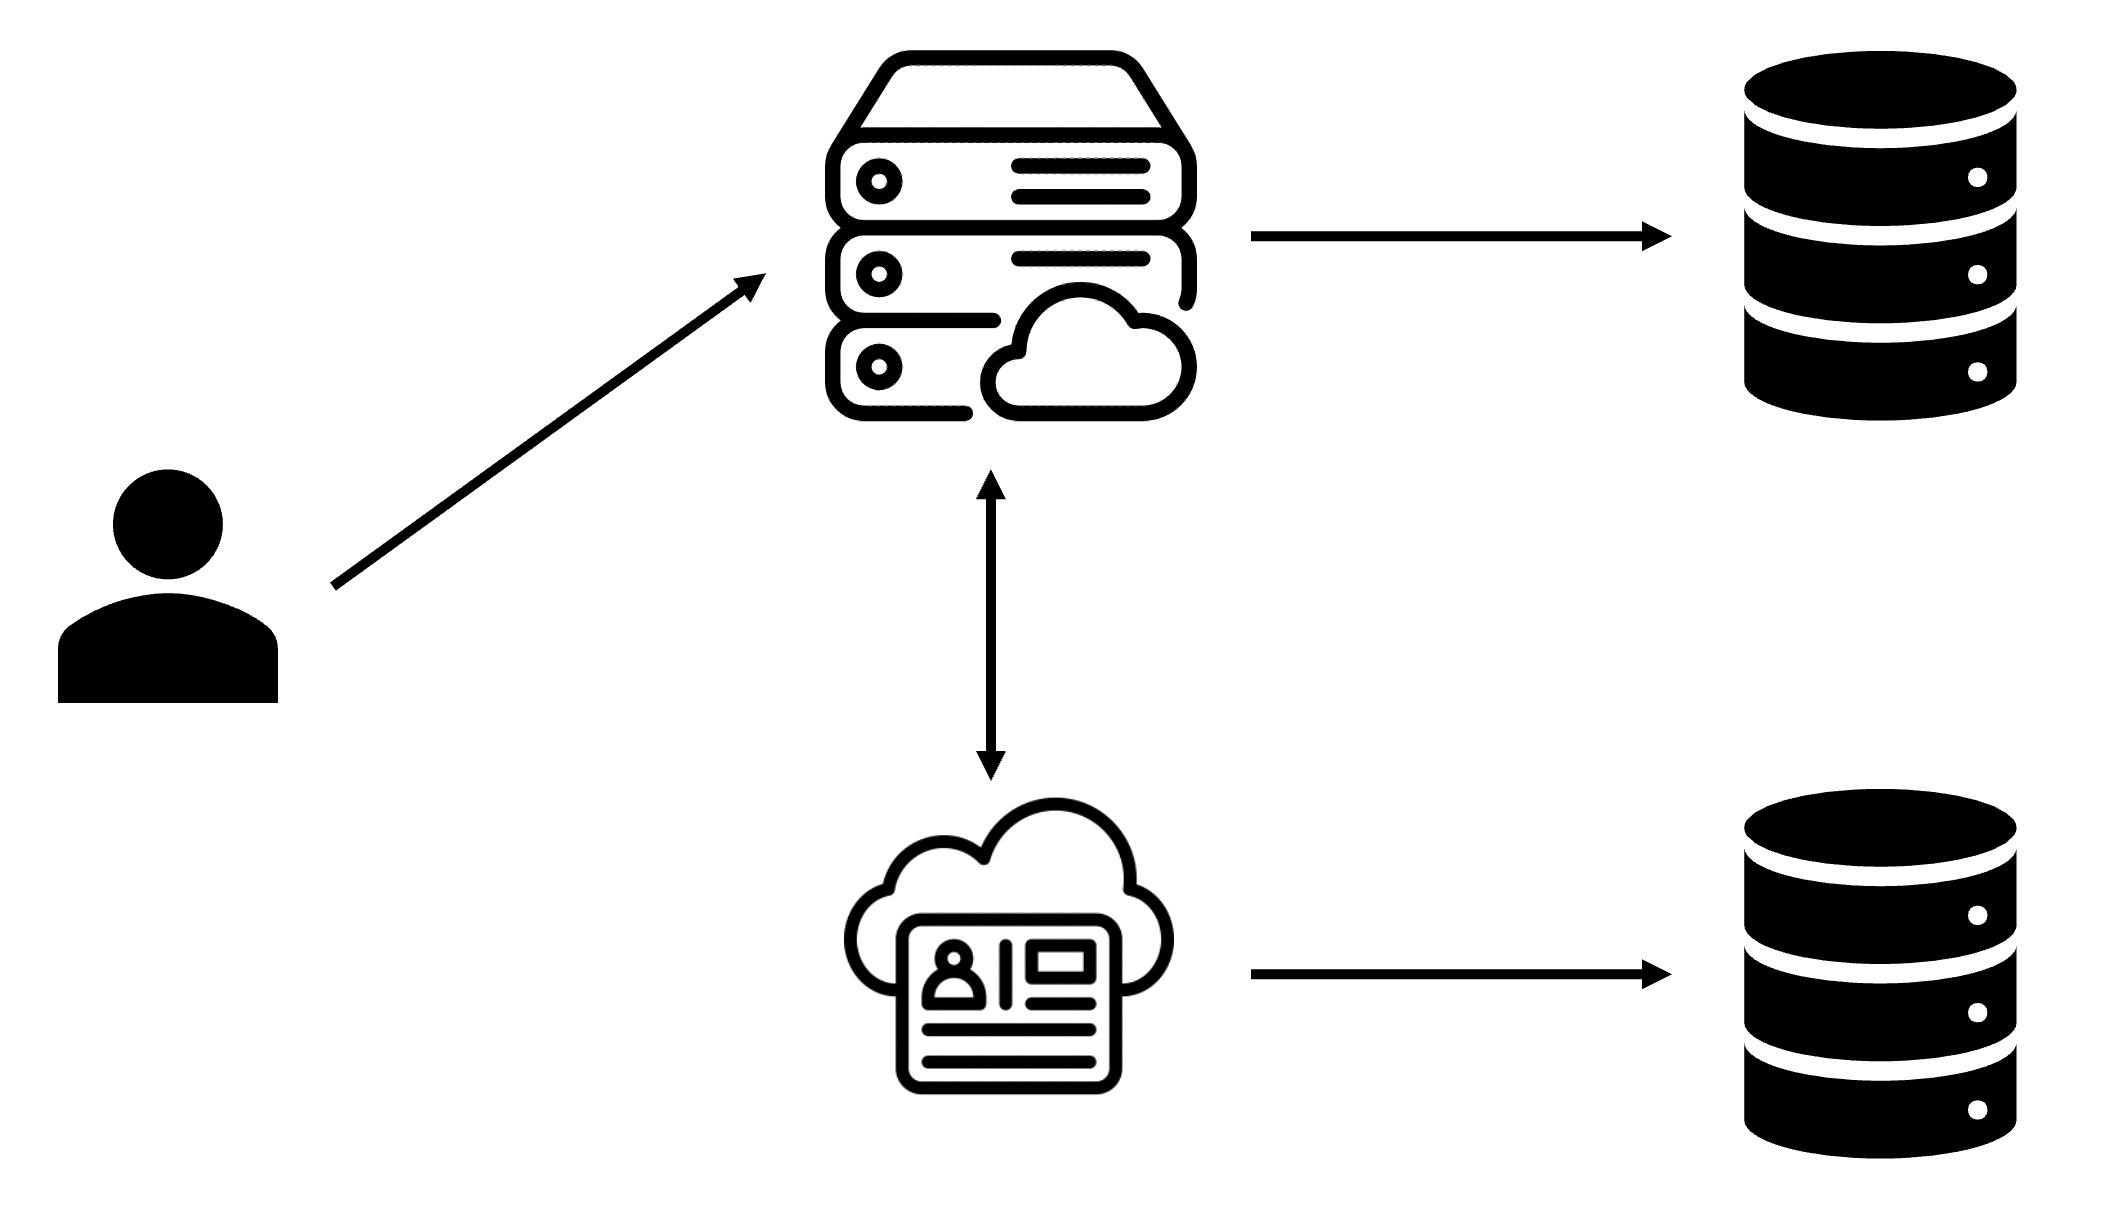
\includegraphics[width=\linewidth,keepaspectratio]{figures/user-mid-identity.png}
  \caption{使用者中心身分}
  \label{fig:user-mid-identity}
\end{figure}
為了解決隱私方面的問題,使用者中心的身分系統如圖\ref{fig:user-mid-identity}所示逐漸興起。這種系統允許使用者透過單一的身分供應者登入多個獨立的服務,同時每個服務各自掌握使用者在其內部的資料。隨著這種需求的增長,新的技術標準應運而生。OpenID和OAuth等協議的出現\cite{sakimura2014openid, hardt2012oauth},標誌著身分管理向使用者賦權的重要轉變。這種模式增強了使用者對個人身分信息的控制權,提供了更大的靈活性,允許使用者選擇不同的身分提供者。

使用者中心的身分系統實現了以服務供應商為單位的資訊範圍控制,在一定程度上改善了隱私保護。然而,這種方式也面臨著一些挑戰。首先是身分碎片化的問題,多個身分提供者的存在可能導致使用者體驗的不一致。其次,安全風險如釣魚攻擊和身分提供者數據洩露等仍然存在\cite{sun2012devil}。此外,儘管使用者獲得了更多控制權,但他們仍然在某種程度上依賴中心化的身分提供者,因此使用者的自主性還擁有很大的提升空間\cite{allen2016selfsovereign}。
\subsection{自治身分}
\begin{figure}
  \centering
  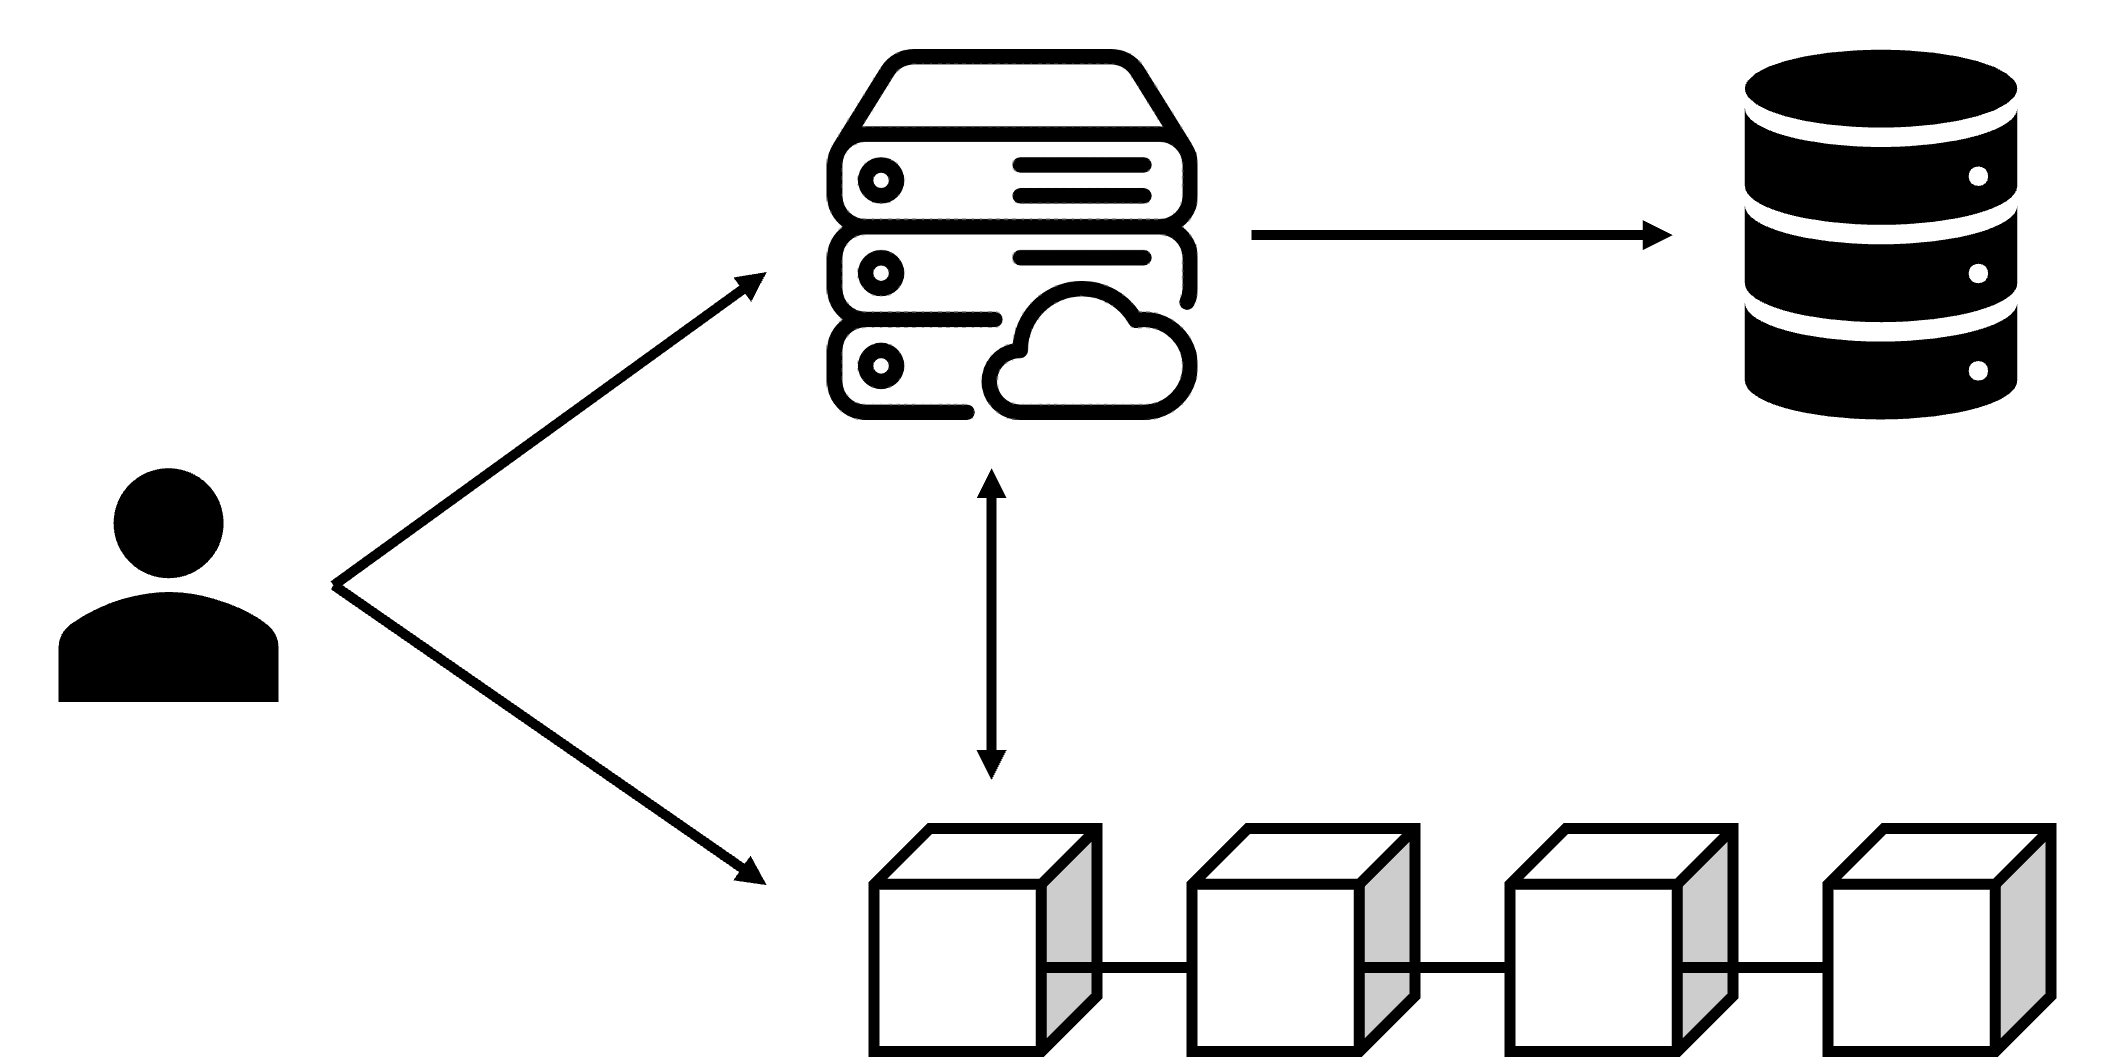
\includegraphics[width=\linewidth,keepaspectratio]{figures/self-sovereign-identity.png}
  \caption{自治身分}
  \label{fig:self-sovereign-identity}
\end{figure}
自治身分如圖\ref{fig:self-sovereign-identity}所示,是身分管理系統的最新發展\cite{preukschat2021self}。這種方式透過區塊鏈技術取代中心化的身分供應商,其代表性例子包括基於以太坊的uPort和微軟的自治身分覆蓋網絡\cite{lundkvist2017uport, microsoft2020ion}。自治身分系統賦予使用者對自身身分的控制權與對身分管理的治理權,同時提高了身分的可攜性和一致性。此外,它還增強了使用者與服務提供商之間的平等性,並提供了抗審查的特性。

然而,作為一種新興技術,自治身分系統也面臨著諸多挑戰\cite{s22155641}:
\begin{itemize}
  \item \textbf{法律框架衝突:} 它可能與現有法律框架存在潛在衝突,例如與GDPR中的被遺忘權不相容\cite{finck2018blockchains}。
  \item \textbf{技術複雜性:} 自治身分系統的技術複雜性可能影響普通使用者的使用體驗,降低其易用性\cite{kubach2020self}。
  \item \textbf{其他問題:} 還有諸如隱私保護、系統互操作性等問題需要解決。
\end{itemize}
\subsection{未來展望}
綜上所述,身分系統的發展經歷了多個階段,每個階段都試圖解決特定的問題。從中心化到使用者自治,身分系統的設計逐漸向使用者賦權,提高了使用者對自身身分的控制權。但是,即使到了使用者自治階段,人們依舊不認為找到了理想的解決方案。如同Schardong等人\cite{s22155641,soltani2021surveydid}所說,當今的自治身分系統仍面臨著許多挑戰,包括安全性、隱私保護、易用性、信任建立等問題。因此,本研究認為身分系統的設計仍有很大的改進空間,需要更多的研究和實踐來不斷優化。
\section{身分系統的困境}
為了設計出一個理想的身分系統,在本節中,會從不同維度的多個方向來探討身分系統的困境。這些討論旨在釐清身分系統的核心特徵,以此為未來的設計提供參考。
\subsection{使用者體驗}
使用者體驗在身分系統設計中扮演著關鍵角色,直接影響系統的可用性和採納率。然而,Hamme等人\cite{inproceedings}的研究闡明了使用者體驗、安全性和隱私保護之間的複雜關係。該研究指出了一個普遍存在的現象:使用者傾向於選擇最簡單的方式來設置和使用身分系統,這種傾向可能導致系統安全性和隱私保護程度的降低。

這種情況產生了一個兩難困境,為了提高安全性而強制使用者採用複雜的身分驗證方式可能會適得其反。例如Zhang等人\cite{zhang2010security}的研究表明,要求使用者定期更改密碼往往導致使用者僅修改特定字元,反而造成更大的安全隱患。同樣地,為了增強隱私保護而要求使用者完成詳細的隱私設置也可能降低使用者體驗。Acquisti等人\cite{acquisti2017nudges}的研究發現,複雜的隱私設置過程往往讓使用者感到困惑和沮喪,甚至導致他們放棄設置而選擇默認選項,從而降低了隱私保護水平。

為解決這一困境,研究者提出了「無摩擦驗證」(Zero Friction Authentication)的概念,旨在最小化使用者在設置和使用過程中遇到的困難,同時維持適當的安全性和隱私保護水平。Hamme等人\cite{inproceedings}強調,無摩擦驗證的核心目標是在保護使用者安全和隱私的同時,顯著降低使用者的操作負擔。這種平衡對於現代身分系統的設計至關重要,因為它直接影響系統的使用率和效能。

為實現無摩擦驗證,近年來安全領域出現了多種新技術。如Ghorbani等人\cite{ghorbani2020fido2}研究了無密碼登入(如FIDO2)的可用性,發現這種方法能透過硬體密鑰在手機上跨裝置完成高安全性的驗證,且使用者普遍認為方便並願意持續使用。Wiefling等人\cite{wiefling2021rba}探討了基於風險的驗證(Risk-Based Authentication,RBA),該方法透過追蹤身分與系統互動的歷史數據,在每次服務請求時動態判斷危險性,並在危險時採用更安全的多因素驗證(Multi-Factor Authentication,MFA)\cite{bonneau2012mfa}。Alaca等人\cite{alaca2016devicefingerprinting}關於裝置指紋的研究顯示,透過在每次使用者對服務發出請求時記錄並比對裝置指紋,可以有效辨識部分惡意行為,且不會增加使用者的操作負擔。

另外,為解決複雜隱私設置帶來的問題,Acquisti等人\cite{acquisti2017nudges}提出了「隱私設計」(Privacy by Design)的概念。這種方法將複雜的設置過程分解為多個簡單步驟,並在使用者使用系統的不同階段逐步引導使用者完成設置。研究表明,這種方法不僅能提高使用者的隱私保護水平,還能顯著改善使用者體驗。

這些新技術的應用表明,在不影響使用者體驗的前提下提供更高的安全性和更好的隱私保護是可能的。然而,如何在自主身分系統中實現真正的無摩擦驗證,以及如何有效地平衡使用者體驗、安全性和隱私保護的需求,仍然是一個值得深入研究的課題。
\subsection{使用者認知}
使用者認知在數位身分管理中扮演著至關重要的角色,直接影響到系統的安全性和有效性。LastPass\cite{lastpass2020psychology}的研究揭示了使用者認知與實際情況之間存在顯著差距:使用者平均估計自己擁有20個線上帳號,而實際上平均擁有37個以上的帳號。這種認知偏差背後反映了使用者使用上的不便,例如經常因為忘記密碼而無法登入帳號,或者因為各個帳號資料不互通而需要耗費大量時間來管理。

Dhamija等人\cite{dhamija2008sevenflaws}的研究進一步指出,使用者對身分管理系統的認知和理解程度直接影響其安全行為。隨著需要管理的使用者名和密碼數量增加,使用者往往感到困惑,進而採取不安全的行為,如使用弱密碼或在多個平台使用相同密碼等。此外,使用者對身分管理系統的認知不足也會導致他們無法有效應對釣魚攻擊、社交工程等安全威脅。

為了解決這個問題,未來的身分管理解決方案應該朝多個方向發展。首要任務是簡化多層次、多維度的使用者身分管理,允許單一的身分管理多樣的別名,以適用於不同的場景。例如,使用者可以用唯一的帳戶創建三個別名,分別對應自己的三種社會身分:在家中是家長,在工作中是員工,在社交場合是朋友。甚至針對單一的服務,使用者也可以擁有多種別名,如在論壇中既可以以專家身分發表權威言論,也可以作為普通使用者表達個人觀點。遵循上述的設計可以幫助使用者在盡可能不增加認知負擔的情況下有效管理自己的身分。

然而,真正簡化使用者認知並非易事。即使是宣稱已解決這個問題的使用者中心身分系統,實際上也未能完全做到。以Google的組織管理文件\cite{gcp2024identity}為例,為了確保不同組織擁有不同的安全限制與規定,系統仍然要求使用者在不同組織間創建不同的身分。這表明,同時簡化使用者認知與滿足組織需求,仍然是一個有待解決的挑戰。
\subsection{隱私保護}
在數位時代,隱私保護已成為身分系統設計的核心考量之一。歐盟制定的《通用數據保護條例》(GDPR)\cite{GDPR2016}代表了目前全球最嚴格的隱私保護標準。本研究認為,一個理想的身分系統應當能夠全面符合GDPR的要求,從而確保使用者隱私得到最大程度的保護。然而,近年來的GDPR違規案例表明,即便是大型企業也面臨著遵守某些GDPR規定的挑戰。

基於Schardong等人的研究\cite{s22155641},本研究發現當前身分系統中存在兩個尤為突出的關鍵問題。首先是使用者積極授權的實現困難。Saemann\cite{saemann2022investigating}的研究強調,在當前的身分系統框架下,企業難以實現使用者對數據使用的明確授權。具體而言,企業難以證明其對數據或權限的使用行為已獲得使用者授權,而使用者也缺乏有效途徑證明自己的數據或權限被不當使用。這種情況不僅增加了企業的法律風險,也削弱了使用者對系統的信任。

第二個問題是被遺忘權的實現困難。Smirnova\cite{smirnova2024understanding}指出,滿足使用者的被遺忘權在當前身分系統中存在著一定的挑戰。使用者數據在系統中往往呈分散狀態,即使刪除核心使用者的資料,仍可能保留使用者的系統日誌或與其他使用者的互動數據。這種情況使得完全實現被遺忘權變得複雜而困難,可能導致使用者隱私無法得到全面保護。

基於以上分析,本研究提出符合現代隱私保護要求的身分系統應該具備兩個關鍵特點。首先,系統應提供合理的機制,讓使用者或企業能夠證明其數據使用行為是否符合授權,這將有助於提高系統的透明度和可信度。其次,系統應提供有效的方法讓使用者行使被遺忘權,確保使用者不會被難以刪除的數據綁架。這意味著系統需要設計更精細的數據管理和刪除機制。在後續研究中,將詳細探討如何在自主身分系統中實現這些特性,並提出相應的技術解決方案。
\subsection{平等信任}
身分系統中的平等信任問題是一個複雜的多方利益平衡問題,涉及系統的公平性和可信度。Alex等人\cite{preukschat2021self}強調了身分系統中各方利益的衝突,主要表現在使用者之間的權益差異、不同系統間的互操作性問題,以及使用者與系統供應者之間的利益衝突。例如,身分系統供應者可能希望獲取更多使用者個人資料以獲取利益,而使用者則希望保護自己的隱私。這種利益衝突如果處理不當,可能導致系統環境惡化、使用者權益受到侵犯,以及市場壟斷和不公平競爭。Zuboff\cite{zhang2010security}的研究進一步指出,這種數據收集和利用的不平等可能導致所謂的「監視資本主義」,對個人自由和社會公平造成深遠影響。

在當前的身分系統中,建立健全的信任模型仍然是一個重大挑戰。傳統的二元邏輯驗證模式(即完全信任或完全不信任)已不能滿足現代身分系統的需求。Schardong等人\cite{s22155641}指出,現實世界的信任往往是模糊而不確定的,人們很難用簡單的真假邏輯分辨使用者是否可以被信任。例如,可能同時存在多個資訊來源,部分認為可信任,部分認為不可信的情況。Josang等人\cite{josang2006exploring}提出的主觀邏輯數學框架為處理這類多組不確定性信任的問題提供了一個系統性的解決方案。該框架將可信度表示為一個區間,從而更好地模擬了現實世界的身分信任過程。

此外,在去中心化系統中,解決身分驗證問題尤其困難。正如Dhamija\cite{dhamija2008sevenflaws}所強調的,使用者需要向系統證明自己的身分,同時系統也需要向使用者證明自己的合法性和可信度。Tze-Nan\cite{NTU202102846}提出的自主憑證機制為解決這一問題提供了一個新的思路。他改良了傳統的憑證簽署(Certificate Authority)技術,使憑證不僅可以由使用者自主操作,還能被所有經手者評分。如此一來,使用者和系統之間就可以在自主的前提下互相驗證並評分,從而建立起一個平等的信任關係。

然而,長期來看,一個合理的評分機制,甚至是一個長期的治理機制也是必要的。在這方面,Chohan等人\cite{chohan2024decentralized}關於DAO(去中心化自治組織,Decentralized Autonomous Organization)治理的研究提供了核心概念,可以為自主身分系統的制度建設提供參考。

在後續的研究中,將探討如何在自主身分系統中實現技術上的互相驗證與制度上的互相信任,最終構建一個能夠平衡各方利益、促進公平競爭而不易壟斷的自主身分生態系統。這種系統將能夠在保護使用者權益的同時,也為系統供應者提供合理的發展空間,從而實現真正的平等信任。
\section{身分系統的評估}
鑒於當前身分系統在各個方面面臨的特定挑戰,本研究提出以下評估標準,用以衡量自主身分系統的設計是否符合下一代身分系統的要求:
\begin{itemize}
  \item \textbf{創新突破}:自主身分系統的設計應解決上節所述困境,才能實現真正的技術創新。以下陳列:
        \begin{itemize}
          \item 使用者體驗:提供無摩擦驗證,簡化操作流程,提高系統易用性。
          \item 使用者認知:提供簡單的身分管理機制,幫助使用者有效管理身分,減少認知負擔。
          \item 隱私保護:實施有效的隱私保護機制,保護使用者個人數據,確保隱私得到充分保障。
          \item 平等信任:建立互相驗證和互相信任的機制,促進所有個體間平等的信任關係。
        \end{itemize}
  \item \textbf{法規遵循}:自主身分系統應符合相關法律法規,特別是在數據保護和隱私保護方面。例如:
        \begin{itemize}
          \item GDPR:遵守一般資料保護規範\cite{GDPR2016}的要求,包括使用者同意、數據可控性和被遺忘權等規定。
          \item NIST:符合美國國家標準\cite{NIST800-63-3},涵蓋多因素驗證、風險評估、身分驗證和授權等要求。
        \end{itemize}
  \item \textbf{公認原則}:遵循身分識別領域的公認原則,包括但不限於:
        \begin{itemize}
          \item 身分法則:符合Kim Cameron提出的身分管理基本法則\cite{cameron2005laws},包括使用者控制、最小化披露和互操作性等原則。
          \item 避免常見缺陷:克服Dhamija等人\cite{dhamija2008sevenflaws}指出的身分管理七大缺陷,如使用者體驗、使用者認知、使用者信任等問題。
          \item 自治身分:符合Allen\cite{allen2016selfsovereign}所說,自治身分應該遵循的10個原則。
        \end{itemize}
\end{itemize}
這些評估標準綜合考慮了技術創新、法律合規性和業界最佳實踐,為評估和設計下一代自主身分系統提供了全面的合理的目標。
\section{本章總結}
本章從身分系統的迭代、設計原則和技術評估三個方面探討了現代身分系統的設計問題。本研究發現,現代身分系統的設計仍面臨著諸多挑戰,包括使用者體驗、使用者認知、隱私保護、平等信任等方面。為了解決這些問題,本研究提出了一系列設計原則,包括無摩擦驗證、隱私設計、使用者認知簡化、......等。在接下來的章節,本研究將進一步探討如何在自主身分系統中達到這些評估標準,並提出相應的技術解決方案。